\newpage
\section{Билет 1. Понятие сплошной среды. Лагранжево и эйлерово описание движения сплошной среды. Индивидуальная производная.}

\defn\textbf{Сплошная среда} - это среда, заполняющая занятую ею область непрерывно, т.е. в любом сколь угодно малом объёме этой области содержится масса.

\defn\textbf{Эйлеровы (пространственные) координаты} - координаты точек среды в системе координат, связанной с пространством, относительно которого происходит движения (пространственной системе координат).

\defn\textbf{Эйлеров подход к описанию движения СС} - величины, характеризующие движение СС, рассматриваются как функции пространственных координат $x^i$ и времени t: $$\vec{f} = \vec{f}(t, x^1, x^2, x^3)$$

\defn\textbf{Лагранжевы координаты} - параметры, которые выделяют индивидуальные точки среды.

\defn\textbf{Лагранжев подход к описанию движения СС} - величины, характеризующие движения СС, рассматриваются как функции времени t и лагранжевых координат $\xi^i$: $$\vec{f} = \vec{f}(t, \xi^1, \xi^2, \xi^3)$$
\begin{figure}[h]
  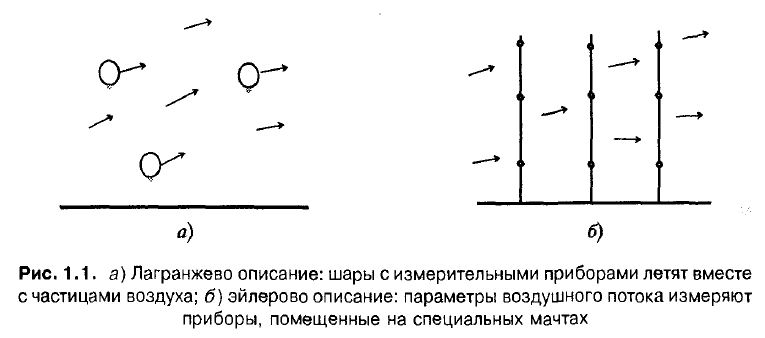
\includegraphics[width=1\textwidth]{01/t1_pic1.JPG}
  \caption{\label{ris:image1_2}1}
\end{figure}

\defn\textbf{Материальная (индивидуальная) производная} по времени от величины f описывает, как эта величина меняется со временем в индивидуальной точке среды. Если f задана в лагранжевом описании, то материальная производная имееет вид (для индивидуальной точки $\xi^i = const $ по определению): $$\frac{df}{dt} = \frac{\partial f(t,\vec{\xi})}{\partial t}$$

Если f задана в эйлеровом описании, то материальная производная имеет вид: $$\frac{df}{dt} = \frac{\partial f(t,\vec{x})}{\partial t} + \frac{\partial f(t, \vec{x})}{\partial x^i}\frac{\partial x^i(t,\vec{\xi})}{\partial t} = \frac{\partial f(t,\vec{x})}{\partial t} + \frac{\partial f(t, \vec{x})}{\partial x^i}v^i$$
